\chapter{Background}
\section{Types of Crosswalks}

There are many types of crosswalks (See figures \ref{fig:TypesOfXwalksFig} and \ref{fig:TypesOfXwalksRealFig} for some examples), the main two are zebra stripe crosswalks (sometimes called 'continental') and standard two line crosswalks. Two line crosswalks are more commonly used due to their simplicity, but zebra crosswalks are often used in more vulnerable intersections due to their benefits in visibility for drivers \cite{crosswalkTypeEvaluation}. Vision processing for the driving lane of a car has been done many times, and there is no substantial difference between that and a two line crosswalk. As such, algorithms that work for these are mostly interchangeable.

\begin{figure}[t]
\begin{center}
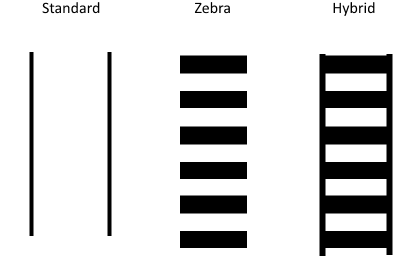
\includegraphics[width=10cm]{figures/TypesOfXwalks.png}
\captionfonts
\caption{A few types of crosswalks}
\label{fig:TypesOfXwalksFig}
\end{center}
\end{figure}

\begin{figure}[t]
\begin{center}
\includegraphics[width=13cm]{figures/All3Types.png}
\captionfonts
\caption{Real world samples of the types of crosswalks}
\label{fig:TypesOfXwalksRealFig}
\end{center}
\end{figure}

\section{Neural Networks}
Neural networks are a type of machine learning that have been used recently for many vision applications such as image classification (See figure \ref{fig:DogWithHat}) and pattern recognition \cite{christianszegedy2014}, because they are useful for datasets with hard-to-detect patterns. Neural networks function using an interconnected network of neurons that work together to process the training data in order to discover a pattern or classification. Neural networks are well suited for many data sets that include lots of information that could be difficult to manually train a computer to categorize. One odd use case for neural networks is that they have been used to help determine which signals from a rat's brain should be used to trigger prosthetic limbs to move by measuring results of brain probes \cite{ratNeural}.

Neural networks are given a large amount of training data with known outputs. The network then runs over the dataset repeatedly, adjusting weighted parameters every iteration to reduce the amount of error in the predictions. Backpropogation of the data is also used in order to assist in training. Once the neural network is trained, the application can feed in new values and receive a prediction of the output.

\begin{figure}[t]
\begin{center}
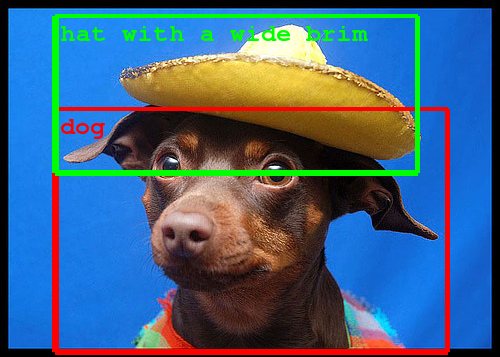
\includegraphics[width=10cm]{figures/DogWithHat.PNG}
\captionfonts
\caption{Neural network classification result\cite{christianszegedy2014}}
\label{fig:DogWithHat}
\end{center}
\end{figure}

%JASON - More in depth than section in background, and more explanation of how they work}
%https://mattmazur.com/2015/03/17/a-step-by-step-backpropagation-example/  (simple example)
%http://home.agh.edu.pl/~vlsi/AI/backp_t_en/backprop.html //more complex example

%Neural networks are a type of machine learning that have been used recently for many vision applications such as image classification (See figure \ref{fig:DogWithHat}) and pattern recognition \cite{christianszegedy2014}, because they are useful for datasets with hard-to-detect patterns. Neural networks function using an interconnected network of neurons that work together to process the training data in order to discover a pattern or classification. Neural networks are well suited for many data sets that include lots of information that could be difficult to manually train a computer to categorize. One odd use case for neural networks is that they have been used to help determine which signals from a rat's brain should be used to trigger prosthetic limbs to move by measuring results of brain probes \cite{ratNeural}.

%Neural networks are given a large amount of training data with known outputs. The network then runs over the entire dataset repeatedly, adjusting weighted parameters of each of the inputs every iteration to reduce the amount of error in the predictions. Backpropogation of the data is also used in order to assist in training. Once the neural network is trained, the application can feed in new values and receive a prediction of the output

\subsection{History}
\label{History}
%http://www.andreykurenkov.com/writing/a-brief-history-of-neural-nets-and-deep-learning/
%http://www.springer.com/cda/content/document/cda_downloaddocument/9789401798150-c2.pdf?SGWID=0-0-45-1495021-p177264210
%yadav_2015

The origins of neural networks originate in 1943, when McCulloh and Pitts published ``A logical calculus of the ideas immanent in nervous activity.'' They showed that simple neural networks could compute a wide array of functions with the same underlying method. A computer that worked as a neural network was created by Frank Rosenblatt and others, with a focus on pattern matching. In 1986, Rumelhard, Hinton and Williams published "Learning Internal Representation by Error Propagation," which popularized the backpropogation method of finding weights, and brought neural networks to the forefront \cite{BackpropHist}, \cite{yadav_2015}.

\subsection{Supervised and Unsupervised Learning}
Machine learning algorithms can be supervised or unsupervised, each with their own uses. Unsupervised algorithms do not have a labeled output, but can attempt to cluster the outputs.  An example of this is trying to distinguish human faces from backgrounds, with a goal of clustering features together. Reinforcement learning is a type of unsupervised learning where the environment rewards good behavior, which leads to that good behavior being repeated. One use case for unsupervised learning is games, because there cannot be a known output. Winning, losing, and gaining points are good examples of reinforcement. 

Supervised algorithms like backpropagation, require a training set with known outputs. Backpropagation works towards a goal of reducing the error so that the predicted outputs are close to the known outputs. Supervised algorithms are useful when the outputs are rigidly defined\cite{SuperAndNotSuper}.

\subsection{Neural Network Basics - Feedforward}
\label{Neural Network Basics - Feedforward}
%example of a simple thing where why the parameters are weighted
The quintessential example of a neural network is a feedforward neural network. This network allows information to move forward only, from the inputs to the outputs. An example of a basic feedforward neural network is shown in figure \ref{fig:smallNN}. A series of weights are assigned to every connection, the inputs are fed through the network, multiplied by each respective weight, summed, and then fed to the next layer until the output values are generated. To train a feedforward network, one must either manually adjust the weights, or come up with a mathematical formula to do so. One such method is backpropagation\cite{feedforwardsource}.

\begin{figure}[t]
\begin{center}
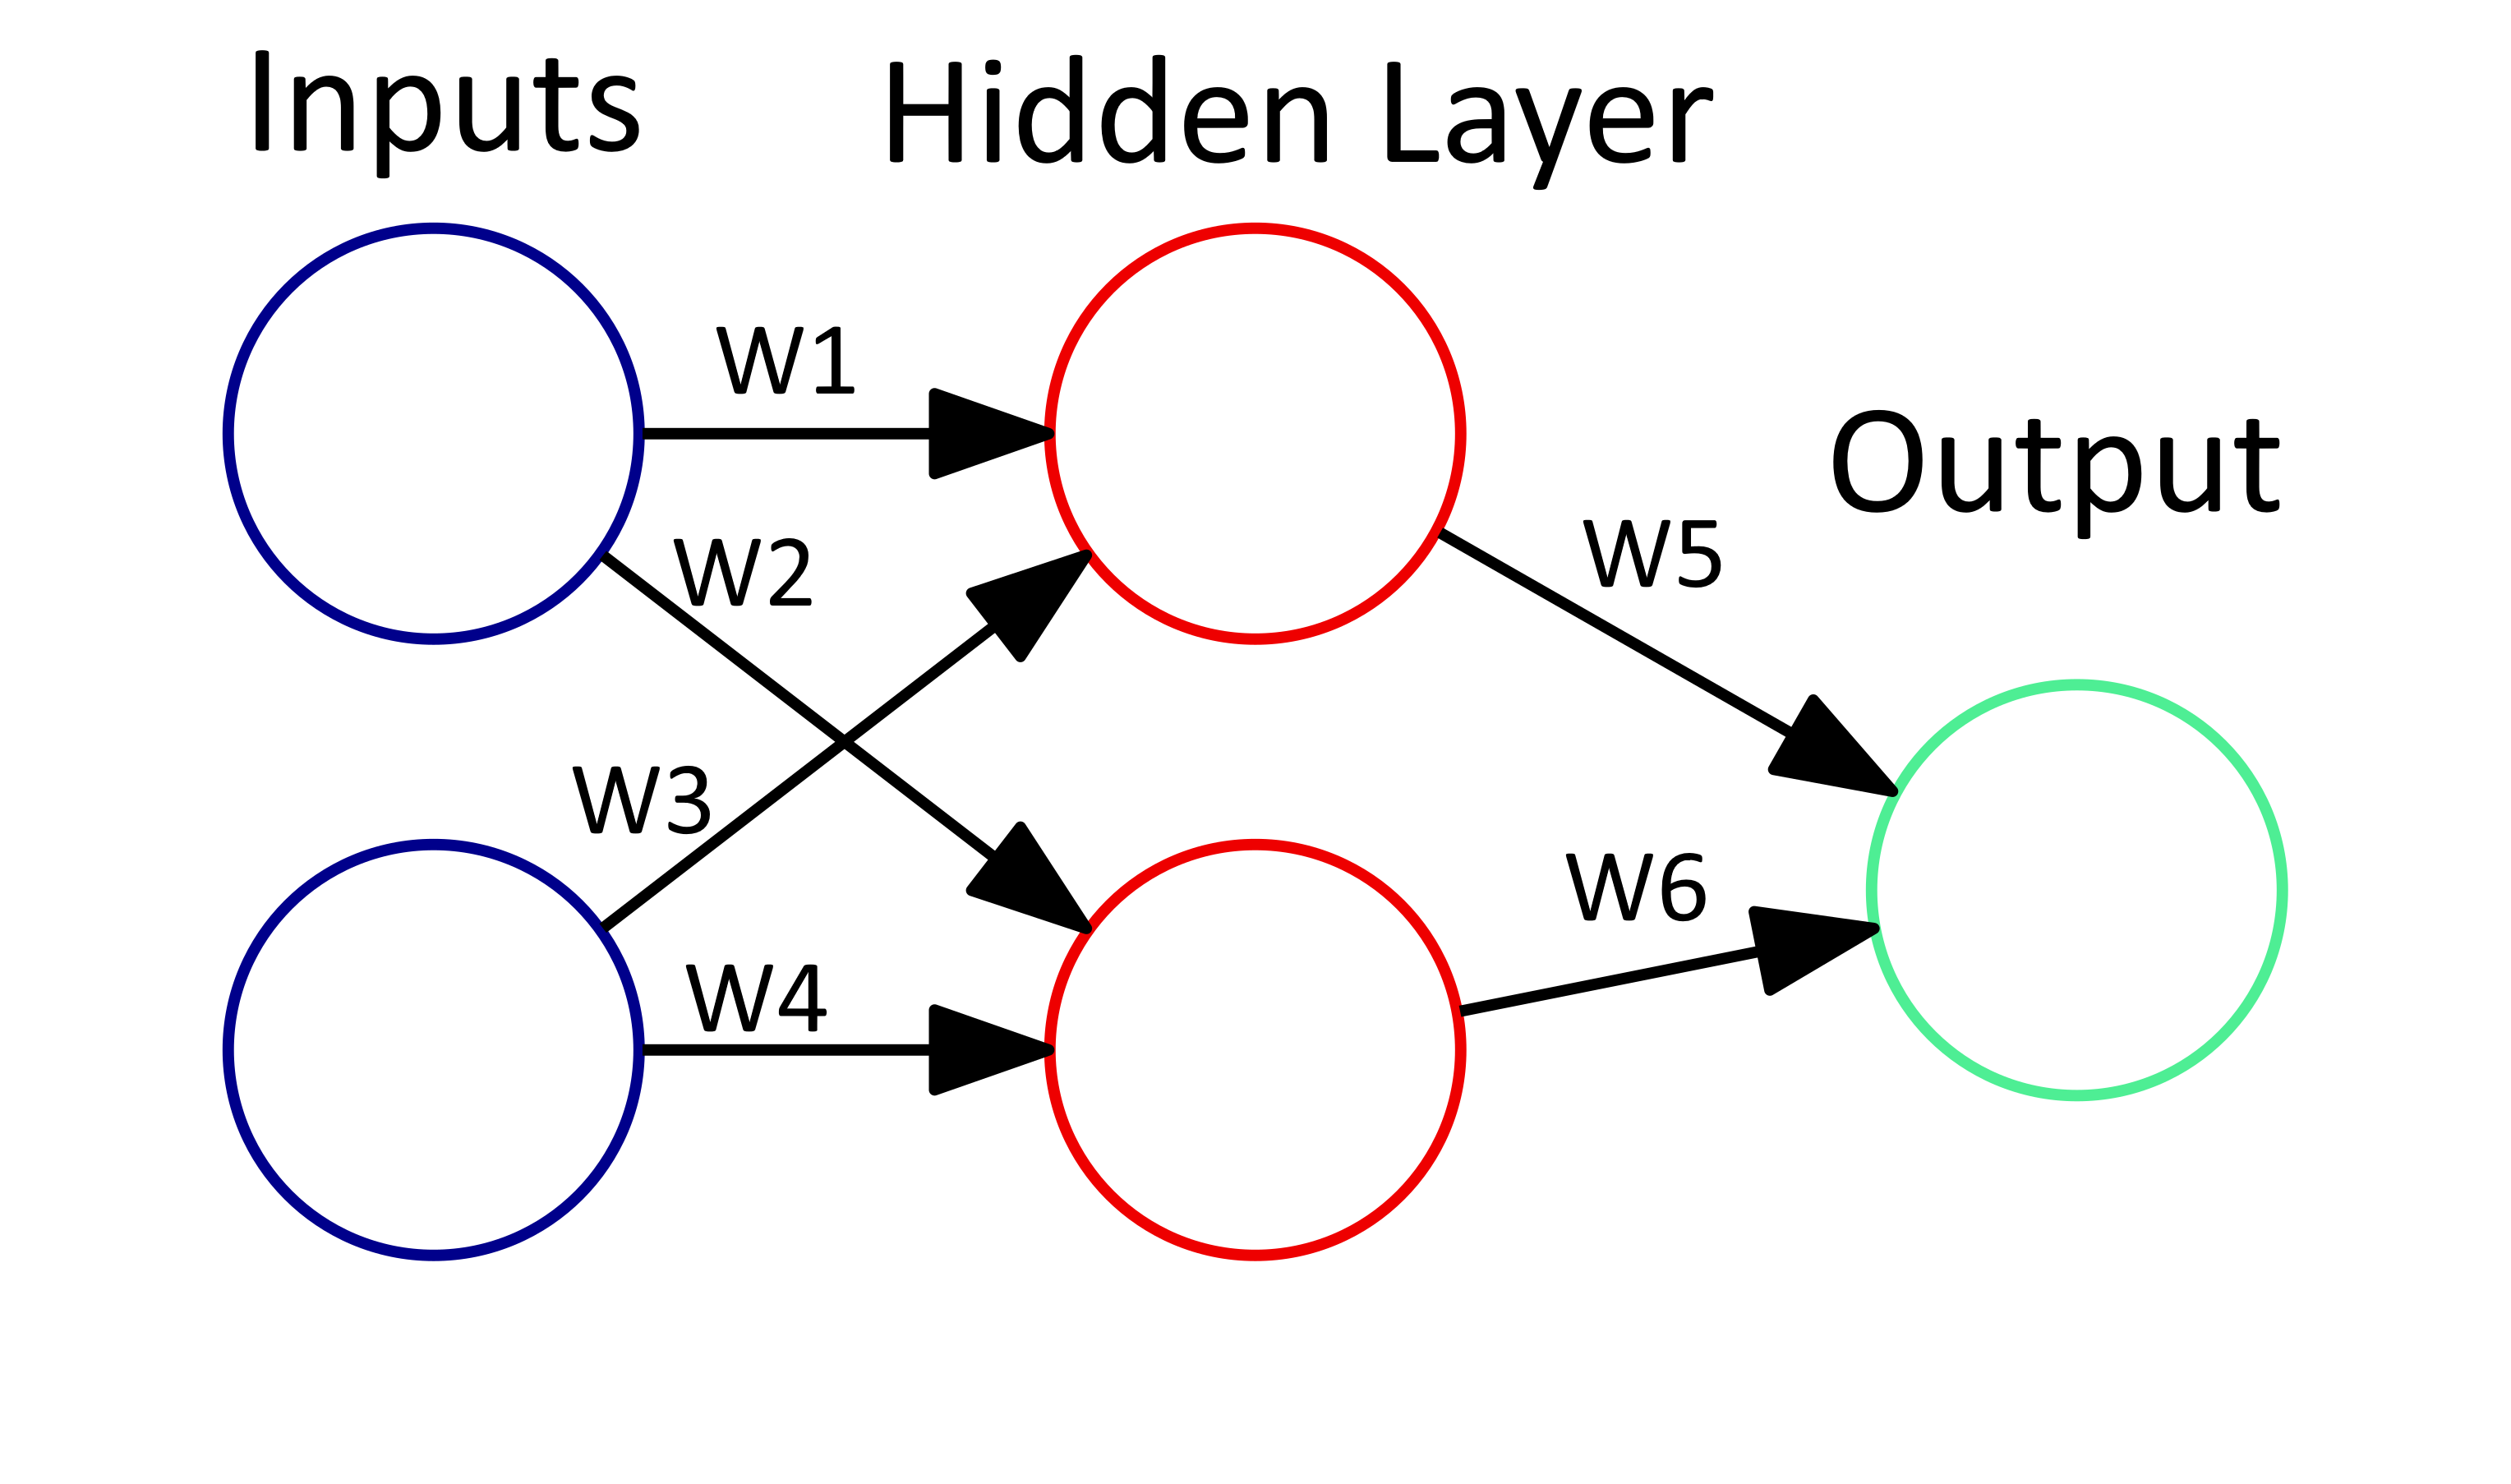
\includegraphics[width=10cm]{figures/simpler.png}
\captionfonts
\caption{Example of a small neural network with weights labeled}
\label{fig:smallNN}
\end{center}
\end{figure}


\subsection{Backpropagation}
\label{Backpropagation Neural Network}
Backpropagation is a method of training neural networks by adjusting weights backwards through the network. It starts with weights for every link, and runs through them. The error on the output is calculated versus the expected output using the squared error function and the sum of the total error among all output nodes. Then, working from the outputs backwards, one works with all of the weights feeding into a prior node one at a time using partial derivatives and the chain rule. The reason the partial derivative is used is because the hidden layers all jointly affect the output nodes' error and must be taken into account. Once all of the weights are adjusted, the error should decrease and then the process is repeated until the error level is reduced to an acceptable level \cite{backpropositionPaper}.